%!TEX root = ../main.tex
\chapter{État de l'art}

Comme vous l'aurez compris, deux sujets principaux seront abordés dans ce mémoire : la gestion de la sécurité informatique
dans une chaîne de production DevOps et la gestion opérationnelle de la sécurité de cluster Kubernetes. 

Il me semble donc pertinent de dresser un état de l'art pour ces deux sujet afin de permettre une meilleur compréhension des
de leurs problématiques, mais aussi afin à mieux appréhender les possibles solutions à ces dernières.

\section{Evaluation des risques de sécurité}
\subsection{Les risques du Pipeline DevOps}

Dans la méthodologie DevOps, le \emph{Pipeline} est un concept regroupant des notions théoriques et socle technique utilisés dans 
le cadre d'un développement logiciel. Ainsi, l'utilisation du terme \emph{Pipeline} fait ainsi reférence au \ac{SDLC}
\autocite[Ch.\ 6]{devops_for_dummies_freeman_forsgren_2019}, aux standards de développement
\autocite[Ch.\ 9]{devops_for_dummies_freeman_forsgren_2019}, processus de qualification et 
validation, de même qu'à l'ensemble des outils et services utilisés par les équipes de développement. Il s'agit donc d'un élément
centrale dans la chaîne de production DevOps: tout problème impactant un élément du \emph{Pipeline} aura des répercutions sur les 
autre et risque ainsi de mettre en péril les opérations de développement.

Nous pouvons donc nous poser la question de la nature de ces risques et particulièrement de ceux relatif à la sécurité du 
\emph{Pipeline}. Pour cela, nous allons utiliser comme support le \ac{SDLC} d'un logiciel afin de mieux cibler les problématiques
de sécurité à chaque étape d'un projet.

\begin{figure}
    \centering
    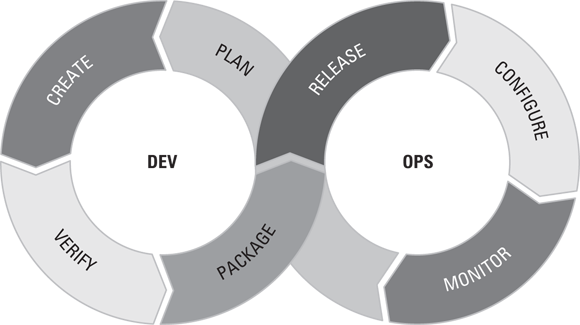
\includegraphics[width=0.5\linewidth]{resources/img/devops_lifecycle.png}
    \caption{Représentation du cycle de vie d'un projet DevOps}
    \label{fig:devops-lifecycle}
  \end{figure}
\newpage

Après une rapide analyse, voici les principaux risque qui se présentes à nous :
\begin{multicols}{2}
    \begin{enumerate}
        \item Plan :
        \begin{itemize}
            \item Intégration d'une technologie vulnérable ou non maintenue
            \item Non-intégration de correctifs pour une vulnérabilité remontée
        \end{itemize}
        \item Create :
        \begin{itemize}
            \item Développement de code faïbles
            \item Mauvaise configuration du framework ou dépendances
        \end{itemize}
        \item Verify :
        \begin{itemize}
            \item Jeux de test incomplets
            \item Absence d'audit de sécurité applicative
        \end{itemize}
        \item Package :
        \begin{itemize}
            \item Utilisation d'un OS ou paquets vulnérables
            \columnbreak
            \item Erreur de configuration du conteneur
            \item Erreur de configuration des services
        \end{itemize}
        \item Release :
        \begin{itemize}
            \item Mauvaise gestion des versions de conteneurs
            \item Erreur de configuration du script de build
        \end{itemize}
        \item Configure :
        \begin{itemize}
            \item Mauvaise gestion des secrets
            \item Erreur de configuration des déploiements
        \end{itemize}
        \item Monitor :
        \begin{itemize}
            \item Absence ou trop faible collecte de log (application et conteneur)
        \end{itemize}
    \end{enumerate}
\end{multicols}

On constate donc que majoritairement les risques sont porté par des erreurs lors du développement et non par
le socle technique de l'application / conteneur. Il s'agira donc d'un point d'attention dans la recherche de
solutions.

\subsection{Les risques d'un cluster Kubernetes}

Bien que l'orchestrateur Kubernetes constitue une coûche d'abstraction entre l'infrastructure physique qui 
l'héberge et les conteneur qu'il fait fonctionner, les risques qu'il porte sont similaires à une infrastructure
(virtualisé ou non) classique. Il est par exemple important de pouvoir lister les instance de conteneur (a.k.a. 
Pod) en cours d'execution, leur version ainsi que la présence de vulnérabilité; de pouvoir assurer un contrôle
d'accès approprié ou bien de pouvoir assurer la sécurité du réseau du cluster. 

Cependant, étant donné que le cluster se comporte comme une coûche d'abstraction, il hérite de problématiques
de sécurité qui lui sont propre. C'est ainsi qu'il est nécessaire de pouvoir surveiller les groupes de ressources
(Namespaces), de contraindre des configuration de déploiement ou l'origine des conteneurs.

